\scanpage{20}
\deleted{iii) Etude du cas où \deleted{$F\unsure{=}$} $a_i=0$ pour $i\geq N+1$, $a_N=1$.

i.e. du cas où
\[
F=Z^N+a_{N-1}Z^{N-1}+\cdots+a_0
\]
les $a_i$ ($0\leq i\leq\unsure{n|N}-1$) nilpotents.
\[
A[Z]/FA[Z]\longrightarrow A[[Z]]/FA[[Z]]
\]
\inserted{base $(Z^i)_{0\leq i\leq N-1}$ sur $A$}
est alors surjectif (car les $Z^i$ ($0\leq i\leq\unsure{n|N}-1$) engendrent $A[[Z]]/FA[[Z]]$ comme $A$-module) je dis que c'est bijectif i.e. que $(FA[[Z]])\cap A[Z]=FA[Z]$ (il revient au $=$ de dire que les \deleted{\unsure{éléments}} $Z^i$ ($0\leq i\leq\unsure{n|N}-1$) forment une base de $A[[Z]]/FA[[Z]]$).
\deleted{Soit donc $a_0+a_1Z+\cdots+a_{N-1}Z^{N-1}$ qui soit multiple de $F$ dans $A[[Z]]$ \unsure{on}.}}
\figure{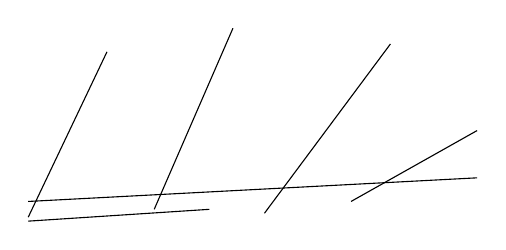
\begin{tikzpicture}[x=1cm,y=1cm]\draw (0,0)--(1,2.1);\draw (1.6,.1)--(2.6,2.4);\draw (3,.05)--(4.6,2.2);\draw (4.1,.2)--(5.7,1.1);\draw (0,.2)--(5.7,.5);\draw (0,-.05)--(2.3,.1);\end{tikzpicture}}

Considérons l'application
\[
\begin{aligned}
\varphi:\quad A^N+A[[Z]]&\longrightarrow A[[Z]]\\
((b_i)_{0\leq i\leq N-1},Q)&\mathbin{-}\sum_{0\leq i\leq N-1}b_iZ^i+QF
\end{aligned}
\]
l'application déduite par passage aux gradués associés pour la filtration $\mathfrak m$-adique (finie) est
\[
(\operatorname{Gr}A)^N\times(\operatorname{Gr}A)[[Z]]\mathbin{-}(\uline{\operatorname{Gr}A})[[Z]]
\]
donné pour un degré $n$ par
\[
((b_i),Q)\longrightarrow\sum_{0\leq i\leq N-1}b_iZ^i+Q\dot F
\]
et comme $\dot F=\deleted{\dot a_{\unsure{N+1|N-1}}}\alpha Z^N$ ($\alpha=a_{N+1}\in A_0^*$) ceci est manifestement bijectif, donc $\varphi$ aussi; cqfd.
\mspage{19}
